\documentclass[12pt]{article}
\usepackage{hyperref}
\usepackage[nottoc,numbib]{tocbibind}
\usepackage[utf8]{inputenc}
\usepackage[acronym,toc,numberedsection=autolabel]{glossaries}
\usepackage{listings}
\lstset{
	basicstyle=\small\ttfamily,
	columns=flexible
	breaklines=true
}
\usepackage{pgfplots}
\pgfplotsset{compat=newest}
\usetikzlibrary{patterns}
\usepackage{svg}

\title{\textbf{Prototyping a Simplified Machine Code File Format For Libraries and Executables}}
\author{\textbf{Author}\\David Gonzalez Martin\\\\\textbf{Thesis advisor}\\Belen Bermejo Gonzalez\\\\\textbf{Coordinating professor}\\Josep Jorba Esteve}
\date{June 2024}
\makeglossaries{}

\newglossaryentry{glibc}
{
	name=glibc,
	description={Short for GNU libc. It is the most standard implementation of libc on Linux.}
}

\newglossaryentry{objdump}
{
	name=objdump,
	description={Program to inspect executable, library and relocatable objects}
}
\newglossaryentry{RIP}
{
	name=RIP,
	description={Short for the instruction pointer register in the x86\_64 architecture.}
}

\newacronym{DLL}{DLL}{Dynamic-link library, Microsoft implementation of a shared library.}
\newacronym{CLI}{CLI}{Command-line interface}
\newacronym{GNU}{GNU}{Recursive acronym: "GNU's Not Unix!"}
\newacronym{GCC}{GCC}{\acrshort{GNU} compiler collection}
\newacronym{BSD}{BSD}{Berkley Software Distribution}
\newacronym{ELF}{ELF}{Executable and Linkable Format}
\newacronym{LLVM}{LLVM}{Low Level Virtual Machine}
\newacronym{PLT}{PLT}{Procedure Linkage Table}
\newacronym{GOT}{GOT}{Global Offset Table}
\newacronym{PIE}{PIE}{Position-Independent Executable}
\newacronym{PIC}{PIC}{Position-Independent Code}
\newacronym{API}{API}{Application Programming Interface}
\newacronym{ASCII}{ASCII}{American Standard Code for Information Interchange}
\newacronym{SIMD}{SIMD}{Single Instruction, Multiple Data}
\newacronym{SSE}{SSE}{Streaming \acrshort{SIMD} Extensions}
\newacronym{AVX}{AVX}{Advanced Vector Extensions}
\newacronym{ISA}{ISA}{Instruction Set Architecture}
\newacronym{NASM}{NASM}{Netwide Assembler}

\begin{document}
	\maketitle{}
	\begin{center}
		
\includegraphics[scale=0.1]{assets/logouoc.png}
	\end{center}
	\newpage
	\mbox{}
	\vfill{}
	\begin{flushright}
		\textit{To my parents, to whom I owe everything.}
		\textit{To my partner, Mariana, who supported and encouraged me in difficult moments.}
	\end{flushright}
		
	\vfill{}
	\mbox{}
	\newpage

	\section*{Abstract}
	\paragraph{}Complexity is present in multiple aspects of modern software development. This work aims to target complexity reduction in the compilation and linking domains. Thus, the main problems that this work is concerned are the unnecessary distinction between static and dynamic libraries and the existence of executable as mere library consumers.
	\paragraph{}To tackle the problem, a new binary format prototype for executable and libraries was developed.
	\paragraph{}This format unifies both library types' ones (static and dynamic) and library and executable ones in a single one. Libraries and executables can either be statically or dynamically linked without the need to previously be compiled for a specific linking mode.
	\paragraph{}Moreover, libraries are provided with entry points to expose related functionality to the user in a convenient manner.
	\paragraph{Keywords:} linking, binary format, static library, dynamic library, executable.
	\newpage
	
	\tableofcontents
	\newpage
	
	\listoffigures
	\newpage
	
	\section{Introduction}
	\paragraph{}Nowadays modern software development has dramatically increased in complexity and both the user and the developer ends experiment problems around it. This work is aimed towards reducing the complexity when directly producing native executable and library binaries.
	\paragraph{}The development of this thesis is fully open-source, so the source code for both this memory and the linker/loader program can be consulted\cite{self}.
	\subsection{Context and Rationale}
	\paragraph{}In modern days there is significant complexity in software, both for the developer and the user. The paradigm for home computing shifted towards web applications as a way to fill the gap that traditional software failed to occupy: cross-platform software. The trend in the developer sector was to forget about memory management and garbage collection started dominating most of common software, especially in the business field. Types were an obstacle to developers, who demanded more and more flexibility, and dynamic typing appeared, leading to the emergence of interpreters and just-in-time compilers.
	\paragraph{}Nevertheless, this cannot only be sensed in the web and business software development world. Systems programming is infected with this fashion as well.
	\paragraph{} The enormous complexity inherited from the times when UNIX was born has generated an overwhelming environment for both users and developers. Code is duplicated or triplicated, leaving the developer with the obligation to deal with more software than necessary and users see how binary files tend to multiply in their disk with no direct corelation with any new feature or improvement whatsoever.
	\paragraph{}Modern compilers and operating systems and complex system software in general are about millions of lines of code, when Linux started out very simple, with just about 20 thousand lines of code. Now the Linux repository is over 20 millions lines of code. Veteran developers like Casey Muratori have criticized the complexity derived of the exponentially increasing lines of code of critical projects\cite{thirty-million}.
	\paragraph{}Another taste of complexity in modern software development: on Linux there are several problems when targetting graphics applications because you cannot link statically since proprietary drivers ship with a specific version of \gls{glibc}. Provided that your system might not provide certain versions of \gls{glibc}, an executable might not run if the version of glibc that was linked with is not located. Linux provides a stable system call interface but this benefit is lost when linking with \gls{glibc}, which is common practice, translating from Microsoft land the so-called term "\acrshort{DLL} hell".
	\subsection{Goals}
	\paragraph{}The general goal of the project is to untangle and reduce the complexity that modern operating systems have between redundant binary components and introduce simple solutions to some of latent problems that the unnecessary separation has been adding.	
	\paragraph{}Some observed issues that would be interesting to tackle in this work are:
	\begin{itemize}
		\item Suppress the distinction between dynamic and static libraries with respect to the file format. A single file can comprehend both and they must not differentiate, giving the chance to the linker to pick the desired linking mode.
		\item Eliminate the distinction between \acrshort{CLI} programs and libraries. Most Linux utilities, like \verb|grep| or \verb|ls|, are standalone programs which link libraries to fulfill their purpose. Instead, the proposal is to have a single binary file which can act both as a library and as an executable.
		\item Allow the user of the format to have different programs hosted inside a single executable. This would allow good capabilities of customization and, what is more important, the following case:
		\item Loader custom logic, allowing the user, among other abilities, to produce an in-memory code section fit for the used CPU architecture, features and instructions.
	\end{itemize}
	\paragraph{}Some of these ideas were already proposed by Jonathan Blow, a veteran programmer, while streaming\cite{jblow}.
	\paragraph{}There are a few ideas which are incredibly temptative to work on, but due to the scope of the project must be unfortunately left aside. Some of the most relevant ones are:
	\begin{itemize}
		\item Implementing a feature system which is both extensible and efficient.
		\item Implementing linking based on integer identification numbers instead of strings or names.
		\item Taking into account security when designing the format. It is a crucial aspect both in modern software and hardware, but again for time reasons must be left aside for the moment.
		\item A good algorithm or implementation to merge sections. Instead, an idea of units or packs will be used.
	\end{itemize}

	\subsection{Impact on Sustainability and Diversity and Social-Ethical Influence}
    \paragraph{} Developing a new executable and library format will yield enormous gains in disk space, which will translate in files being in the operating system filesystem cache more frequently and thus leading to faster program loading and less CPU cache pollution. All of this will translate to less energy consumed by computers, but not only because of the previous factors mentioned. Correct CPU instruction selection is crucial to save both energy and time, as professor Daniel Lemire states \cite{lemire-energy}. 
	\subsection{Used Method and Approach}
	\paragraph{}This work will only be addressing the x86\_64 architecture along with the \acrshort{GNU}/Linux operating system, for a matter of simplicity and time limitation. For the same reason, no existing libraries will be used. The source will be written in Zig\cite{zig}, a new systems programming language. The version of Zig used will be the nightly or master release, which can be downloaded from here\cite{zig-download}. For a pinned release version, \verb|0.13.0-dev.351+64ef45eb0| successfully builds and runs the project.
    
    \paragraph{}The skeleton of the project will be a program which works both as a linker and as a loader, it being able to generate binaries, load them from disk and resolve relocations, as well as setting them up for execution.
    
    \paragraph{}At the same time, current executable and library formats will be examined to look for good concepts to integrate into this more modern format and bad practices to be avoided.
    
    \paragraph{}Moreover, relocation types will be examined with a critical approach. Part of the complexity had in binary formats which contain native code is the wide range of unnecessary features. The investment in such features is widespread and unfortunately such practice is normalized.
    
    \paragraph{} With respect to the production of the relevant machine code, manual encoding will be used despite the existence of a few production-ready assemblers for x86\_64. 
    
    \paragraph{} The reasoning behind of all these decisions will be described in detail in the next sections.

	\subsection{Planning}
	\paragraph{}The necessary resources to elaborate the project were:
	\begin{itemize}
		\item Zig toolchain\cite{zig}
		\item \acrshort{GCC}\cite{gcc}
		\item \acrshort{LLVM}\cite{llvm}
		\item \acrshort{NASM}\cite{nasm}
		\item defuse.ca online assembler and disassembler\cite{online-assembler}
		\item Godbolt\cite{godbolt}
	\end{itemize}
	
	\paragraph{}With respect to the tasks that need to be completed in order to achieve the proposed goals, here they are listed by order:
	\begin{itemize}
		\item Research on the matter of linking and executable and library formats.
		\item Code a basic linker/loader which can serialize to disk and load to memory.
		\item Support a standalone library with entry point
		\item Support a standalone executable
		\item Support a dynamically linked executable
		\item Support a statically linked executable
		\item Support CPU dynamic dispatch extension and several programs into a file.
	\end{itemize}
	
	\subsection{Thesis Overview}
	The main proposal of this work is to develop a prototype of a machine code format for both libraries and executable, aiming to simplify the current state of affairs. This targets the suppression of duplicities such as executables versus libraries, dynamic versus static linking, different relocation types and merging altogether, object format versus executable/library format, etc.
	
	\newpage
	\section{Resources and Approach}
	
	\paragraph{}Since the target of this work is the x86\_64 architecture and the \acrshort{GNU}/Linux operating system, the research on the state of affairs is going to be as well on the formats used by this platform, that is, the \acrshort{ELF} specification and the System V ABI (for x86\_64).

	\subsection{A Brief Exploration of ELF}
	
	\paragraph{}\acrshort{ELF} is a binary file format used by Linux and other UNIX-like operating systems, such as the \acrshort{BSD} family and Solaris, among others.
	\paragraph{}In what follows, different particularities of ELF which are relevant to this research will be described.
	
	\subsubsection{Types of ELF Files}
	
	\paragraph{}According to the \acrshort{ELF} specification\cite{elf-spec}, there are three main kinds of \acrshort{ELF} files, also called by the spec as \textit{object} files:
	\begin{itemize}
		\item A relocatable file, which is supposed to be linked to other objects afterwards.
		\item An executable file, which can be used for direct execution.
		\item A shared object file, which may be used both to produce a bigger object file by linking to other objects or, primarily, can be linked at runtime with an executable file by the dynamic linker, and these are indexed by the program headers.
	\end{itemize}
	\paragraph{}However, by examining the \verb|e_type| field of the \acrshort{ELF} header data structure, aside from the main types (\verb|ET_REL| for relocatable files, \verb|ET_EXEC| for executable files and \verb|ET_DYN| for shared object files), there is another type of file supported under the \verb|ET_CORE| tag, which refers mainly to core dumps.
	
	\subsubsection{Sections and Program Headers Duality}
	
	\paragraph{}\acrshort{ELF} files classify data into groups by means of both sections and segments.
	\paragraph{}Data in sections refer to all information valuable to the linking process and they are indexed by the section headers.
	\paragraph{}On the other hand, the data contained in the program segments contain all the information needed for constructing the process or executable image, that is, the bytes that need to be in memory in order for the program to work properly.
	\paragraph{}\acrshort{ELF} being a general-purpose format, it has to support a wide variety of use cases in both the section and program headers.
	\paragraph{}Therefore, section headers have to support cases with no apparent utility, such as null sections. Others types supported are very specific to certain cases, which are included in this bloated scheme of linking the equally swolen web of code. The paradigmatic case of this is again the \acrshort{GNU} libc. To exemplify the amount of sections, an optimized executable (non-stripped) built with Zig and linking a few \acrshort{LLVM} libraries has the following sections, most of which have to do with \gls{glibc} and dynamic linking\cite{nativity}:
	\begin{verbatim}
0 .interp
1 .note.ABI-tag
2 .dynsym
3 .gnu.version 
4 .gnu.version_r
5 .gnu.hash
6 .hash
7 .dynstr
8 .rela.dyn
9 .rela.plt
10 .rodata
11 .eh_frame_hdr
12 .eh_frame
13 .text
14 .init
15 .fini
16 .plt
17 .tbss
18 .init_array
19 .data.rel.ro 
20 .dynamic
21 .got
22 .got.plt
23 .relro_paddin
24 .data
25 .bss
26 .comment
27 .gnu_debuglin
28 .debug_loc
29 .debug_abbrev
30 .debug_info
31 .debug_ranges
32 .debug_str
33 .debug_line
34 .debug_pubnames
35 .debug_pubtypes
36 .debug_frame		
	\end{verbatim}
	
	\paragraph{}At the same time, the specification says that program headers have exclusive utility for shared objects and executables, leaving out relocatable files.
	\paragraph{}Program headers are similar to section headers, only that they tend to group section data into categories according to whether the section must be loaded by the \acrshort{ELF} dynamic linker or loader and similar criteria. For instance, there is \verb|PT_LOAD| that informs that the object segment must be loaded into memory, \verb|PT_DYNAMIC| collects dynamic linking information and \verb|PT_INTERP| is used as the path to an interpreter, to mention a few.
	
	\subsubsection{A Sea of Relocations}
	\paragraph{}Relocations as such are described in a very generic way, which two (\verb|Elf64_Rel|) or three (\verb|Elf64_Rela|) generic fields. The relocation type is encoded as part of the \verb|r_info| field and is architecture-dependent.
	\paragraph{}Since this work only deals with the x86\_64 CPU architecture, such part of the specification will be examined.
	\paragraph{}Nevertheless, the original \acrshort{ELF} specification, despite including information for Intel architectures, is previous to the creation of x86\_64, so another document must reached in order to retrieve some certain data about the relocation types for the flagship architecture of Intel and AMD.
	\paragraph{}However, the existence of the relocation data in the original document can help the interested reader understand the growing complexity of linking technology. By the time the \acrshort{ELF} specification was published, there were only three possible encodings for relocation types, two of which were actually relocations (where one exists with respect to the program counter).
	
	\paragraph{}The picture is indeed quite different when looking through the document which properly describes the relocation types for the newer x86 extension for, the AMD64 or x86\_64 System V ABI specification\cite{x86_64-abi-spec}. If there were only three options for relocation type in x86, for AMD64 there is a total amount of 38 possible values to encode. This, aside from the increasing complexity of types, has to do with the addition of different sizes, not only the 64-bit one but also 8-bit and 16-bit relocations. By paraphrasing Cliff Click's great work on compilers\cite{sea-of-nodes} in a pejorative sense, it can be concluded that there is a "sea of relocations" in x86\_64.
	
	\subsubsection{Dynamic Linking and Lazy Bindings or Sticking Code Together with Too Much Glue}
	
	\paragraph{}The ploriferation of relocations was accompanied by an increasing complexity in the relationship between different pieces of the code that ought to be linked. The appearance of intermediate linking tables such as the \acrshort{GOT} and the \acrshort{PLT} introduced unnecessary intermediate steps to a dynamic linking stage already hurt in performance.
	
	\paragraph{}Part of the complexity and overhead introduced by dynamic linking is introduced by lazy bindings\cite{lazy-bindings}. When these are used, the function call to a dynamically-linked symbol jumps into a stub in the \acrshort{PLT} section. This \acrshort{PLT} stub then jumps into yet another stub, this time in a \acrshort{GOT} entry, responsible for loading the symbol on demand using the \verb|dlsym| function from libc. Once the symbol is loaded, \acrshort{GOT} entry is updated with the symbol address.
	\paragraph{}This approach ensures that only the symbols that are actually used are loaded, avoiding huge work if large libraries are linked. Nevertheless, the penalty for each symbol load is worse, since the linking of the library cannot be batched.
	\paragraph{}The performance penalty of calling a dynamically-loaded function can be summed up by a couple of jumps (from the calling code to the \acrshort{PLT} and from the \acrshort{PLT} to the actual function) and an extra memory dereference (the function address contained in the \acrshort{GOT} entry), provided that the function is not called for the first time. This could signify the presence of a few unnecessary cache misses as opposed to the simple \verb|call| with a \gls{RIP}-relative operand.
	\paragraph{}This triple indirection poses an obvious penalty and thus dynamic linking with lazy bindings features meaningful overhead in both speed and size.
	
	\subsection{Simplification of Executable Formats}
	\paragraph{}In previous subsection, a concise explanation was provided regarding the complexity of \acrshort{ELF}. The aim of the current subsection will be to provide a faithful comparison between the existing format and one aligned with the goals outlined in this study.
	\paragraph{}Most of the problems drafted before will be addressed and proposals which match the study goals will be made.
	
	\subsubsection{Executables and Libraries}
	
	\paragraph{}The separation between executable and libraries is irreconciliable in the \acrshort{ELF} format. Any library, which has already passed the linker stage, cannot offer an arbitrary execution of code.
	\paragraph{}The main purpose to offer a library to execute an arbitrary piece of code is to offer the user some functionality related to what the library provides when linked. Thus the user could receive some functionality directly from the library, and not needing any third-party executable with the library linked.
	\paragraph{}This is common in all major operating systems. Since the target of this work is the Linux operating system, an instance of this issue is the melting pot of command line programs offered in their distributions, such as \verb|coreutils|. 
	\paragraph{}A library with some related functionality which could be accessed through an entry point would avoid this needless complexity, putting together grains of sand with similarities.
	\paragraph{}This would report some disk space savings (since there is no need for separate files) and better load times (there is a trend in the Linux userspace to dynamically link these executables in order to save some space).
	\paragraph{}Such modification requires some deep changes in the whole linking/loading structure, since the kernel would need to recognize library entry points in order for all users to enjoy this feature without any added complexity.  So aside from a format change, this would also require patching the binary loader in the kernel and probably the dynamic linker as well.
	
	\subsubsection{A Hate Letter to Shell Scripts for Composability}
	
	\paragraph{}In the previous section some thoughts were expressed regarding substituting command-line executables with libraries with user-facing functionality (mainly oriented towards satisfying shell users, but not only them).
	\paragraph{}However, the preferred method to join functionalities in an operating system should be via the linker, that is, linking binary code and data together to perform one or more functionalities. Both dynamic and static libraries report noticeable gains in terms of speed and size over the UNIX manner of commanding the computer to execute one binary after another through scripting.
	\paragraph{}In a way, shell scripting is little more than a contenation of executable runs which communicate together through text ---\verb|stdin|, \verb|stdout|, \verb|stderr| and the corresponding pipes--- with a few added conveniences).
	\paragraph{}To expand the idea, the so-called \textit{convenient} composability of shell scripting turns against developers in a reasonably sized project for two main reasons:
	
	\begin{itemize}
		\item Lack of static typing and checking, which helps catching errors before even the first execution is made and it ensures the intention of the author was genuine. The absence of it could hide bugs in unexplored code paths which might trigger in production environments.
		\item Slowness, due to:
		\begin{itemize}
			\item A considerable amount of separate \acrshort{ELF} objects need to be loaded into memory to make up a collection of programs which achieves a \textit{single} program's functionality. This triggers filesystem cache misses and puts onto the computer an unnecessary burden for the sake of the human convenience, which at the end of the day might not be entirely true.
			\item The communication protocol between these pieces of a program (since a shell script is actually a glorified program) is text, which is known to be far from efficient. Computers understand about numbers and bytes and not human characters.
		\end{itemize}
	\end{itemize}
	
	\subsubsection{Help the Fastest Also Be Flexible: Overcoming the False Dicotomy of Static and Dynamic Libraries Before Linking}
	\paragraph{}Once the idea for composability is clear enough, there are multiple of aspects of \acrshort{ELF} that do not comply with this project goals. One of them is related to linking mode preceding linking when it comes to libraries.
	\paragraph{}Currently, \acrshort{ELF} does not admit to choose the mode a library is linked with once it is produced. If someone wants to link dynamically some library, it must be compiled with that in mind. On the contrary, if the choice is static linking,  the same behavior must follow.
	\paragraph{}However, it is not written in stone that one should pick the linking mode before producing the desired binary file.
	\paragraph{}One of this project goals is to uniform the binary format, not only libraries with executables, but libraries with themselves. A dynamic library file should have the same bytes in disk that a static version of it. Accordingly, the linking choice can be postponed until linking time (which, when read, makes total sense).
	
	\subsubsection{Rescuing Dynamic Linking from the Complexity Mud}
	\paragraph{} As stated in the \acrshort{ELF} overview, the complexity, though generalized, primarily manisfests within dynamic linking.
	\paragraph{}The existence of sections such as the \acrshort{GOT} and \acrshort{PLT}, together with lazy bindings, suffocates this linking mode by making it slower and more bloated, when it was precisely originated with the opposite purpose in mind.
	\paragraph{}Furthermore, the traditional separation between static and dynamic libraries was frequently manifested with different relocation types, making the artificial gap between them larger.
	\paragraph{}Dynamic libraries tend to make more use of the compiler \acrshort{PIE}/\acrshort{PIC} code generation option, while static libraries tend to honor its qualifier.
	\paragraph{}However, there is no reason to think that they cannot share the relocation type. In fact, the same way the dynamic linker patches \acrshort{GOT} entries, it can directly patch the symbol address in all the references to it. This way, a relocation relative to the instruction pointer can be used for both linking modes. In x86\_64, there are multiple relocation sizes of this kind, so the 32-bit one will be used for the sake of simplicity. 32-bit should be enough, given that most code/data will be in a 4 GB range.
	\paragraph{}The benefit of uniforming the relocation type and eliminating \acrshort{GOT}, \acrshort{PLT} and lazy bindings is that dynamic code no longer have triple indirection but performs about the same than static code. This, however, comes at the cost that no lazy symbol loading can be done and patches are needed on a per symbol reference basis, not on a per symbol existence one as before.
	\paragraph{}However, these disadvantages are not that important when they are measured in the eyes of this work's guidelines: bloated libraries are discouraged and they are the main beneficiaries for lazy bindings. At the same time, since modern CPUs are up for batches and bandwidth, patching the same symbol relocations repeated times across the binary must not pose a serious problem.

	\subsection{Machine Code Generation}
	
	\paragraph{}There are multiple manners to produce machine code. It should be clear that the code is not generated to fulfill an user demand or functionality. This code is generated so that relocations can be easily located and patched.
	\paragraph{}The typical one would be to use a compiler, which translates high-level language source code into machine code. However, the author of the code does not have control on the byte output but as a merely optimizer advisor.
	\paragraph{}Another plausible option is to use an assembler, which receives the text representation of the machine code as input and also produces machine code. Nevertheless, it has the same problem as the compiler use case: the user has no control over what bytes are generated and where the relocations start and end.
	\paragraph{}Finally, the last explored option, which ended up being the chosen one, was to emit the machine code by encoding the instruction bytes directly. This option gives the best control over the code generated to the programmer, who is in charge of every byte of machine code. Relocation start and ends (therefore sizes as well) are known.
	\paragraph{}This has the disadvantage of not being very scalable and the code generated is not worthwhile aside from being food for the linker and the loader. Yet the goal of this work is to research linking and loading technology, not to produce useful code to be linked or loaded, so the trade-off is acceptable.
	\paragraph{}The instructions in this work are encoded directly, as mentioned above. However, although the author feels somewhat familiar with x86\_64 encoding, the task has been performed with the help of an assembler. As a disclaimer, the encoding of the instructions is not intended to be a full-fledged assembler, but rather the necessary tool for the task at hand.
	\paragraph{}There are a couple of resources which assisted me greatly in this regard.
	\paragraph{}The first one is an online assembler for x86 and x86\_64\cite{online-assembler}. It internally uses \acrshort{GCC} and \gls{objdump} to transform the assembly source code into encoded bytes.
	\paragraph{}The second one is Godbolt, a website which is great to explore code optimization and generation\cite{godbolt}. The last one allows to choose the programming language, the compiler and its invocation arguments as well as extra visualizations.
	\paragraph{}On the other hand, Zig is a nice language that lets you execute most of the code at compile time (as long as they can be executed in a virtual machine with no target-specific instruction or function call). While complicated \verb|comptime| (the keyword in Zig for compile time execution) code will not be used, some samples are listed following this paragraph to show what Zig is capable of in this regard, remarking the fact that Zig has no preprocessor within their tools:
	
	\begin{itemize}
		\item The bytes to returning 32-bit zero in x86\_64. Here the \verb|++| operator works to concatenate arrays at compile time.
		\begin{verbatim}
const xor_eax_eax = [_]u8{0x31, 0xc0};
const ret = [1]u8{0xc3};
			
const ret0 = xor_eax_eax ++ ret;
		\end{verbatim}
		\item A function to generate the encoding of a 32-bit \verb|mov| to the general-purpose register \verb|eax|, which can be invoked at compile time:
		\begin{verbatim}
fn mov_eax_imm32(imm32: u32) [5]u8 {
	return [1]u8{0xb8} ++ @as(*const [4]u8, @ptrCast(&imm32)).*;
}
		\end{verbatim}
		\item At last, the whole function to generate the encoding for the main function (the entry point), shared for both the library and executable samples from the testbed.
		\begin{verbatim}
const main_print_library_code = 
// Set up the stack
mov_rsp_rdi ++
// Call the function to get the number
// (this contains an unresolved relocation)
call(0) ++
// Format the decimal digit as an ASCII character
// (this number is inside a 32-bit register)
add_eax_imm8('0') ++
// Mov the 32-bit into the data section
// so that it can be printed (this contains an unresolved relocation)
mov_rip_mem_eax(0) ++ 
// 1 - write syscall id
mov_eax_imm32(1) ++
// 1 - file descriptor: stdout
mov_edi_imm32(1) ++
// Move that character buffer pointer
// as first argument (this contains an unresolved relocation)
lea_rsi_rip_mem(0) ++ 
// 1 - stdout file descriptor
mov_edx_imm32(1) ++
// write(stdout, &buffer, 1);
syscall ++
// exit(0);
xor_edi_edi ++
mov_eax_imm32(231) ++
syscall;
		\end{verbatim}
	\end{itemize}

	\paragraph{}These are the relevant bits in regard to machine code generation. When generating the executable, these bytes are appended to the code section. A similar approach is followed when generated non-code section data. For example, when generating a symbol in the data section, the desired bytes for symbol are written in the same fashion to the end of the section.
	\paragraph{}For relocations, as stated before, 4 bytes will be used. Unresolved relocations will leave the 4-byte operand as zero. The location of the patch will depend on the type of relocation: if it is internal (where the target symbol is located in the same binary unit) or external (for instance, the target symbol belongs to another file). Internal relocations take no metadata space in disk since they can be resolved before writing the binary file to disk or loading a program to memory. External relocations belong to their own section.
	
	\subsection{Loader and Linker Implementation}
	
	\paragraph{} On most operating systems (and Linux is no exception), the executable loader belongs in the kernel. Unfortunately, the scope and time limitation for this project make it impossible to face such a 
	change in addition to the ones already done.
	
	\subsubsection{Executing a program from userspace in a virtual memory system}
	\paragraph{}Still, there is an option on modern systems to achieve a similar result from userspace invoking the virtual memory system \acrshort{API}. This is, to reserve and commit a region of virtual memory with special permissions, so that it's possible to execute code from that region.
	\paragraph{}Such functionality is fulfilled by the \verb|mmap| system call on Linux\cite{mmap} and POSIX systems. A roughly equivalent \acrshort{API} on Windows is provided by \verb|VirtualAlloc|\cite{virtual-alloc}. An additional benefit of this system call is that, if the correct flags are specified, the memory is private to the process and is zero initialized. Thus the way to accomplish a functional loader and linker is to use this \acrshort{API}.
	\paragraph{}This \acrshort{API} could be used in separate parts, by first reserving the memory (using the \verb|PROT_NONE| flag) and then committing using a different system call, \verb|mprotect|, which allows to change the protection flags for an specific virtual memory region that has already been reserved. While this \acrshort{API} is useful to have pointer-stable arrays which require no copy when growing, the usefulness for this work 
	is limited and the author will stick to the first option.
	
	\subsubsection{Linker and Loader Code Overview}
	
	\paragraph{}In the prototype of linker and loader developed for this work, there are some funcionalities that needed to be covered:
	\begin{itemize}
		\item Given some inputs, serialize to disk a file with the new format containing the desired code and data. This functionality is covered by the \verb|write_binary| function.
		\item Link a binary (\verb|link|). Library/object inputs are described in the executable itself, so the linker is able to pick it up, open the corresponding file from disk and include the necessary functionality in the final binary. This works for both static and dynamic linking. In the case of static linking, the binary can be optionally serialized to disk.
		\item Loading functionality, from both memory (\verb|load_from_memory|) and disk (\verb|load_from_disk|). This uses the aforementioned method to allocate virtual memory with execution permissions.

	\end{itemize}
	\paragraph{}In the following subsections these three parts of the implementation will be described more in detail.
	
	\subsubsection{Producing a Binary File}
	\paragraph{}
	The function \verb|write_binary| receives as inputs:
	\begin{itemize}
		\item The output file path.
		\item An array of sections, each of them containing:
		\begin{itemize}
			\item An array of symbols, each of them formed by a name and the content in bytes.
			\item The section id, which can be one the following: \verb|code|, \verb|data|, \verb|internal_table|, \verb|data|, \verb|internal_table|, \verb|external_table|,\\ \verb|relocations|, \verb|symbol_table|, \verb|string_table|, \verb|library|.
			\item Read, write and execute flags.
			\item An alignment attribute which defaults to 4.
		\end{itemize}
		\item An array of internal relocations, which is information for the linker to resolve before writing the file to disk or loading the binary for execution.
		\item An array of libraries to be imported, each of them containing its name and a list of symbol names to be imported.
		\item An array of external relocations referenced by the unit/module code, to be resolved later at linking stage.
		\item A reference to the entry point, represented by the symbol and section indices.
		\item An enumerator to indicate whether the binary is an executable or a library.
	\end{itemize}
	\paragraph{}Given this set of inputs, the \verb|write_binary| function is able to encode a working binary. In addition, it will resolve internal relocations and generate the convenient extra sections, such as the symbol and string tables.
	
	\subsubsection{Linking Binaries Together}
	\paragraph{}The \verb|link| function serves as a dynamic and static linker, since the procedure is identical.
	\paragraph{}The main file to be linked is read from disk, although it could easily be adapted to operate directly from memory.
	\paragraph{}First, the section headers are iterated in search of interesting sections to perform the linking.
	\paragraph{}Once they are examined, it is checked that if relocations exist, an external table exists and vice versa. On the contrary, if there are not any relocations, there must not be an external table and vice versa.
	\paragraph{}If there are any relocations to be made, the pertinent content from the interesting sections is fetched and relocations are iterated over.
	\paragraph{}For each relocation, the following steps are taken:
	\begin{itemize}
		\item Fetch the destination library name and symbol name.
		\item Search through the libraries that are already cached to find by name.
		\item If the library is not already cached, load it from disk and add them to the list of cached libraries. Append it to the final file buffer (for the time being the binaries are linked altogether).
		\item Fetch relevant sections from the library (string and symbol table).
		\item Search through the symbols by name.
		\item When found, obtain the necessary data to perform the relocation and make it as if it were internal. Break the symbol search loop, jumping back to the loop header to perform a new relocation iteration if applicable.
	\end{itemize}
	
	If the user provides a path, then the \verb|link| function must write the binary to a file with the specified path.
	
	\subsubsection{Loading Functionality}
	\paragraph{}This functionality is the most straightforward of the three. A couple of functions are provided to load from file and from memory.
	\paragraph{}The first similarity is utilizing a virtual memory region with execution permission to load the full file to it. Note that in order to load a binary for execution, the file must be fully linked, so there must be no relocations in it.
	\paragraph{}Part of loading an executable is also providing a stack the code loaded can use. For this reason, a new call to \verb|mmap| is made to allocate a decent amount of memory (this time without execution permission).
	\paragraph{}In the end, the header is fetched and the entry point address is computed and cast into a function pointer with \verb|noreturn| return type. It was not worth the trouble to be able to return from the binary (since this is the natural behavior of executables, they do not return), so the exit procedure is fully contained inside the binary. This way, any code from the linker/loader after the jump to the binary is made will not be run.
	
	\subsubsection{A Simple Testbed}
	\paragraph{}The samples for testing are two, an executable and a library.
	\paragraph{}The dummy functionality used as a testbed is to provide a function which returns 5 as a 32-bit integer. This code belongs to the library. Both the executable and the library contain a shared (in the sense that the code is roughly the same) entry point function which interoperates with this library function. Roughly speaking, the entry point calls the library function to obtain the desired number, formats it into \acrshort{ASCII}, stores it into memory and prints the number to \verb|stdout|. The detailed steps are the following:
	in the following manner:
	\begin{itemize}
		\item The stack is set up from the \verb|rdi| register.
		\item Call into the library function (if it comes from the executable, such relocation is external; otherwise, internal).
		\item After the call, the return value is inside the \verb|eax| register, so in order to format it as an ASCII character, it needs to be added to the value for \verb|'0'|.
		\item Once the number is formated in \acrshort{ASCII}, it is stored into the data section memory (in order to print to \verb|stdout| the number, it needs to reside in memory). For this memory address an internal relocation is needed.
		\item When the value is properly stored, the syscall arguments are prepared and the CPU is told to run the \verb|syscall| instruction itself.
		\item Finally, another syscall is made to exit the process.
	\end{itemize}
	
	\paragraph{}Since libraries in this format can have an entry point associated with the related functionality the library itself provides, the test entry point is shared in both the executable and the library, with the unique difference of the relocation kind.
	\paragraph{}When the executable is linked, the linker must pull the library from disk and link it against the executable. If the library is produced, only the internal relocation needs to be resolved and no call to the \verb|link| function is needed, since the \verb|write_binary| function resolves any internal relocation.
	
	\paragraph{}Below some help regarding on how the codebase can be tested is provided.
	\paragraph{}To write and execute only the library, the \verb|execution_type| constant must be set to \verb|Header.Kind.library|.
	\paragraph{}On the other hand, to produce both the executable and the library and link them together, the \verb|execution_type| constant must be set to\\ \verb|Header.Kind.executable| (this is the default value).
	\paragraph{}Another choice is given when linking the executable: whether it should be linked statically or dynamically. Such option is controlled by the constant \verb|linkage|. To go for static linkage, the value of this symbol must be \verb|Header.Linkage.static|. On the contrary, for dynamic linking, the required value is \verb|Header.Linkage.dynamic|.
	\newpage
	
	\section{Results}
	\paragraph{}The code that has been developed throughout the semester is able to produce:
	\begin{itemize}
		\item A standalone traditional library and a standalone traditional executable that, though not listed as specific goals, are implicit goals which need to be achieved in order to show more interesting functionality.
		\item A library which can also work as an executable (by having an entry point related to the binary functionality).
		\item A library which can be linked either dynamically or statically starting from identical bytes, meaning that a separate or dedicated file is not needed for each linking mode.
		\item An executable which can be loaded into memory dynamically linked or which can be statically linked, generating a different file with every symbol needed contained in the same file.
		\item The dynamic linker does not put unnecessary indirections between code from different libraries or units.
	\end{itemize}
	
	\paragraph{}The goal of this work was to be compared in performance when generating these files, since the tools used for the job are pretty rudimentary and far from ideal for a production environment worth looking into. Given this fact, it is hard to measure a battle-tested production-ready compiler with a tiny prototype which is only able to assemble and compile a couple of test files.
	\paragraph{}While this is true, a comparison draft in terms of size, so some data could be thrown into the light to somehow materialize the achievements of this research.
	
	\subsection{Binary Size Reduction}
	\paragraph{}The next programs will be used to prepare the comparison, listed along their versions:
	\begin{itemize}
		\item \acrshort{GCC} 14.1.1
		\item Clang 17.0.6, C compiler of the \acrshort{LLVM} toolchain.
		\item ld 2.42.0
		\item \acrshort{NASM} 2.16.03
		\item \gls{glibc} 2.39
	\end{itemize}
	
	\paragraph{}To be able to compare the result in size with existing solutions, a few configurations were selected in order to generate similar code to the one used in the testbed:
	\begin{itemize}
		\item \acrshort{GCC} using system library (\gls{glibc}) dynamically and statically linking.
		\item Clang using system library (\gls{glibc}) dynamically and statically linking.
		\item \acrshort{NASM} producing a standalone object statically linked.
	\end{itemize}
	
	\paragraph{}To uniform the test cases, no debug information is going to be generated by any compiler or assembler. Moreover, linker invocations are always guaranteed to use the strip-all flag (\verb|-s|) and section garbage collection (\verb|--gc-sections|)\cite{man-ld}.
	\paragraph{}Compiler invocations will optimize with the \verb|-Oz| flag to aggressively optimize for size\cite{man-clang}.
	\paragraph{}While it could have been interesting to compare different libc implementations, like musl\cite{musl}, since most likely they could have done a better job than \gls{glibc} in that matter\cite{libc-comparisons}, they are not as easy to integrate\cite{how-musl} as the dominant \gls{glibc}, which is present in almost every Linux distribution given their affiliation with the \acrshort{GNU} organization and their legacy\cite{glibc}.
	\paragraph{}Source code for the C and assembly implementations which are compared to the code developed for this thesis can be found in the \verb|test_against| directory from the project root source tree.
	\paragraph{}Libc implementations will use the \verb|fputc| function to print to stdout.
	\paragraph{}Next, different configuration commands will be listed:
	\begin{itemize}
		\item \acrshort{GCC} with dynamic linking (\gls{glibc}):\\
		\verb|gcc -o main ../library.c ../main.c -Oz -Wl,-s -Wl,--gc-sections|\\
		Binary size: 14344 bytes.
		\item \acrshort{GCC} with static linking (\gls{glibc}):\\
		\verb|gcc -static -o main ../library.c ../main.c -Oz -Wl,-s -Wl,--gc-sections|\\
		Binary size: 682424 bytes.
		\item Clang with dynamic linking (\gls{glibc}):\\
		\verb|clang -o main ../library.c ../main.c -Oz -Wl,-s -Wl,--gc-sections|\\
		Binary size: 14368 bytes.
		\item \acrshort{GCC} with static linking (\gls{glibc}):\\
		\verb|clang -static -o main ../library.c ../main.c -Oz -Wl,-s -Wl,--gc-sections|\\
		Binary size: 690720 bytes.
		\item \acrshort{NASM} static executable without libc:\\
		\verb|nasm ../nasm.S -felf64 -o nasm.o|\\
		\verb|ld nasm.o -o nasm -s --gc-sections -static|\\
		Binary size: 8472 bytes. By using the linker \verb|-n| flag, it got down to 4568 bytes.
		\item This work (dynamic linking) (executable.nat file):\\
		Binary size: 299 bytes.
		\item This work (static linking) (static.nat file):\\
		Binary size: 536 bytes.
	\end{itemize}
	
		\begin{figure}
		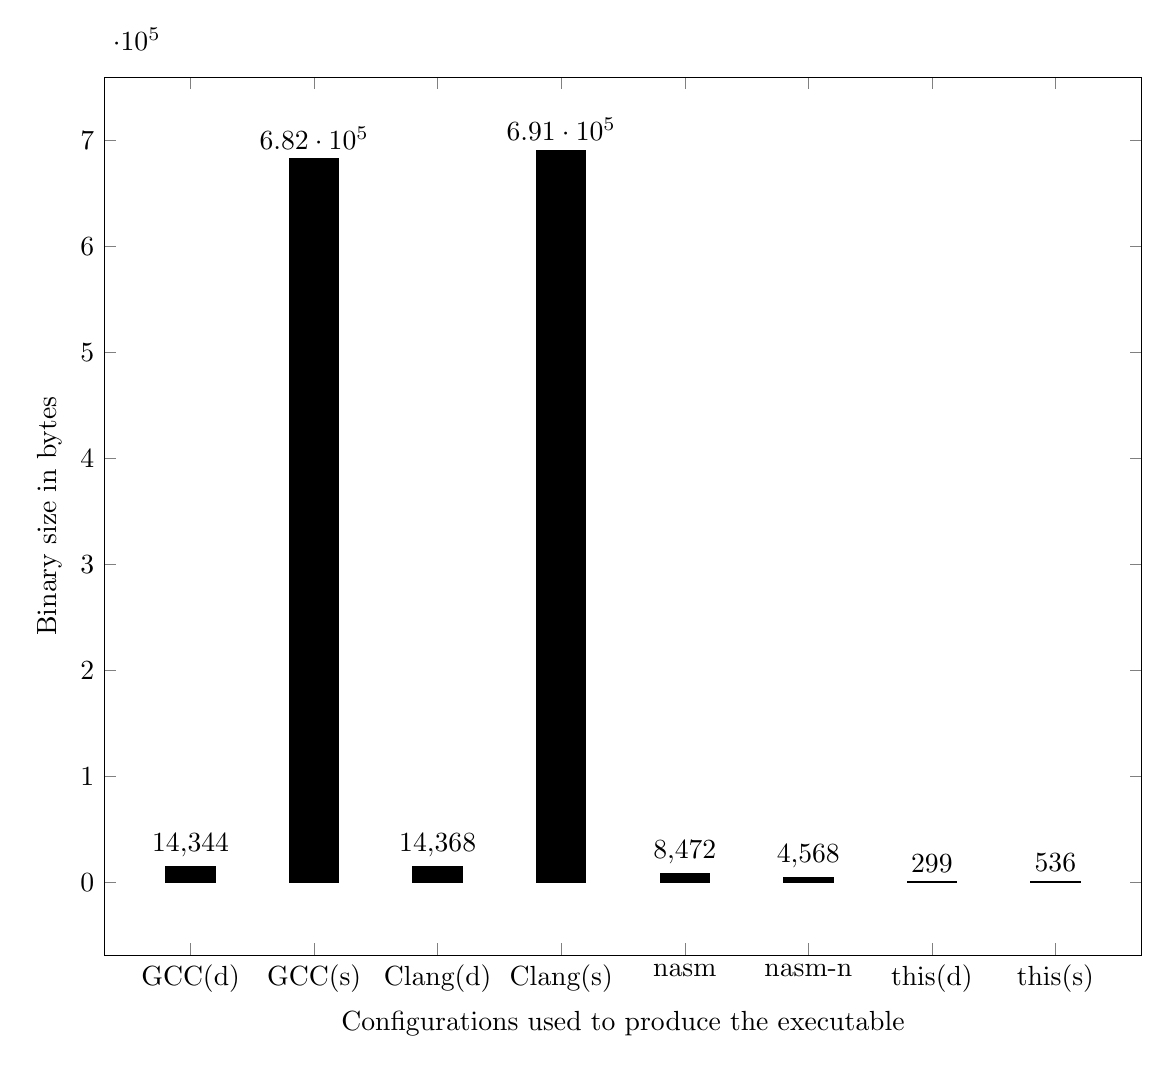
\begin{tikzpicture}
			\begin{axis}[
				xtick={1, 2, 3, 4, 5, 6, 7, 8},
				xticklabels={GCC(d),GCC(s),Clang(d),Clang(s),nasm,nasm-n,this(d),this(s)},
				width=420,
				ylabel={Binary size in bytes}, xlabel={Configurations used to produce the executable}, nodes near coords, bar width=0.4]
				\addplot[ybar,fill=black] coordinates {
					(1,14344)
					(2,682424)
					(3,14368)
					(4,690720)
					(5, 8472)
					(6, 4568)
					(7, 299)
					(8, 536)
				};
			\end{axis}
		\end{tikzpicture}
		\caption{Full comparison of executable sizes}
		\label{fig:full-comparison}
	\end{figure}
	
	The results are depicted on figure \ref{fig:full-comparison} (\verb|d| stands for dynamic, \verb|s| for static, \verb|-n| for \acrshort{NASM} object linked with the \verb|-n| flag and the binaries produced by the research are referred as \verb|this|).
	
	\paragraph{}The most noteworthy aspect about figure \ref{fig:full-comparison}  is that glibc static executables are gigantic in comparison to the others. Although it is a library that can be linked statically, this is not practical because glibc is meant to be dynamically linked, since it uses a lot of calls to \verb|dlopen| in order to set things up. A number of issues can be found related to this \cite{so-static-glibc}\cite{fasterthanlime}.

	\begin{figure}
		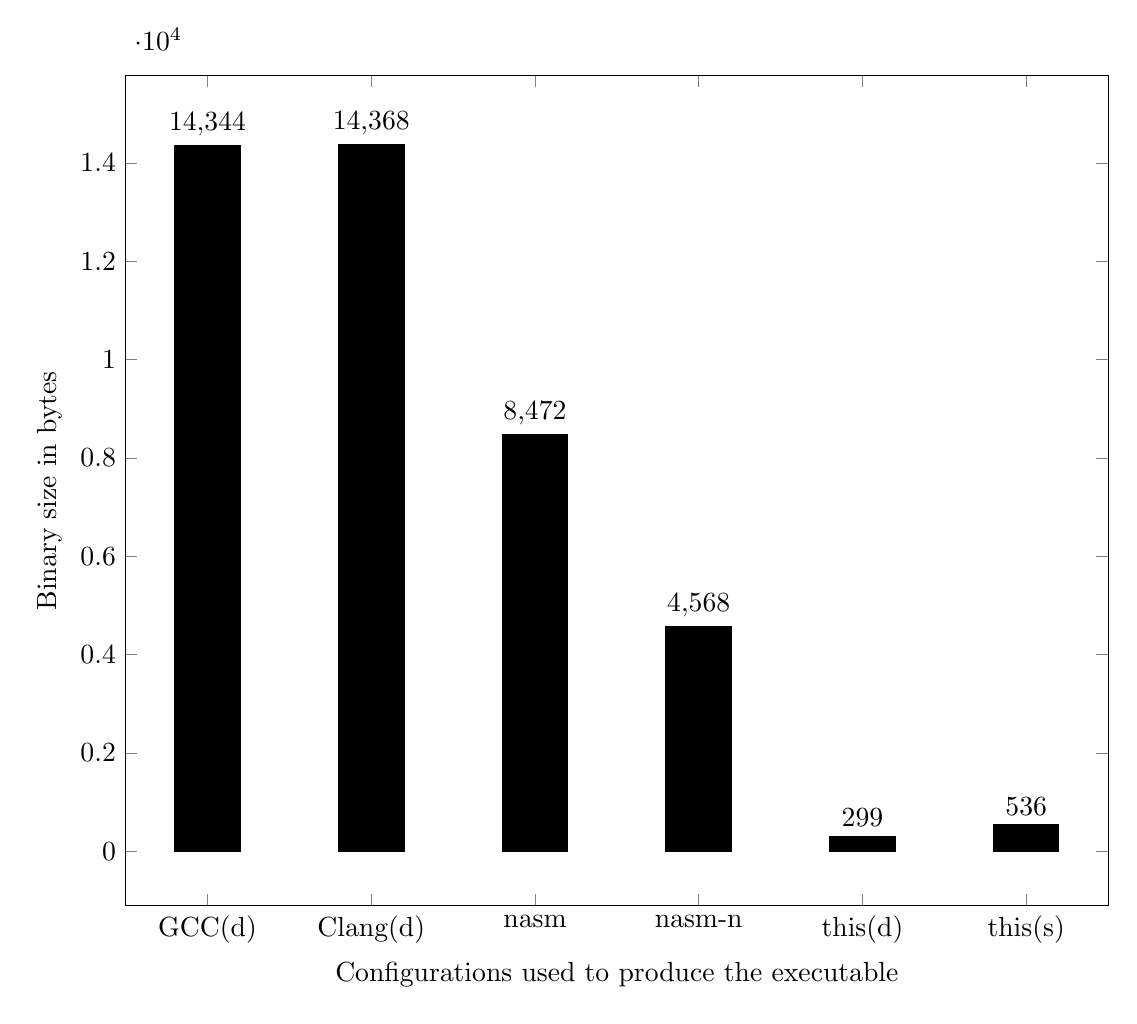
\begin{tikzpicture}
			\begin{axis}[
				xtick={1, 2, 3, 4, 5, 6},
				xticklabels={GCC(d),Clang(d),nasm,nasm-n,this(d),this(s)},
				width=400,
				ylabel={Binary size in bytes}, xlabel={Configurations used to produce the executable}, nodes near coords, bar width=0.4]
				\addplot[ybar,fill=black] coordinates {
					(1,14344)
					(2,14368)
					(3, 8472)
					(4, 4568)
					(5, 299)
					(6, 536)
				};
			\end{axis}
		\end{tikzpicture}
		\caption{Comparison of executable sizes without the glibc static ones}
		\label{fig:pruned-comparison}
	\end{figure}
	
	\paragraph{}On figure \ref{fig:pruned-comparison}, the static glibc executables are left out of the equation.
	\paragraph{}A noticeable matter is that linkers by default are obliged to maintain a 4K page alignment for sections. However, the \verb|nasm-n| version commanded the linker to remove that restriction and, though it reduced the binary size almost in half, it still has some margin of improvement. It was nonetheless impossible to apply this linker flag to gcc and clang binaries because it gave several errors complaining about not being able to find libgcc that could not be resolved.
	\paragraph{}On the other hand, one could remark how much smaller the executables generated by this work's code are. The smallest \acrshort{NASM} executable was roughly 8.5 times the size of the static executable and more than 15 times the size of the dynamic one.
	\paragraph{}Comparing them to the dynamic glibc executables, which are the most common in C and C++ code nowadays, the Clang dynamic binary was almost 27 times the size of the static version and 48 times the size of the dynamic one.
	\paragraph{}An obvious conclusion follows: there was an important size reduction in binary size, even though the merging algorithm for the linker was far from efficient.
	
	\subsection{Resolving the Problem of Executables as Library Consumers}
	\paragraph{}With respect to the library with entry point functionality, the goal was accomplished successfully, having the possibility to potentially reduce binary file count and disk size by a lot. While this is true, some test results were not possible to provide, since this would require the new format to be deployed at scale in order to appreciate the delta.
	
	\newpage
	\section{Conclusions}
	\paragraph{}This humble work is nothing but a grain of sand towards a better future for computation.
	\paragraph{}Once the size measurements have been compared to battle-tested production-ready developer tools and have proven to be competetive even if the developer time is infinitely inferior to the amount of work put in giant codebases like \acrshort{GCC} or \acrshort{LLVM}, a satisfaction must come out of it.
	\paragraph{}The current state of affairs in software development is massively overcomplicated and that there were huge chances to do better. Software development has been made artificially more complicated by humans when trying to coarsely fit the constructs of the human mind in totally different systems such as computers.
	\paragraph{}Although the expectations for this thesis were a little big higher, personal difficulties and time limitations have constrained the amount of goals that were initially aimed to be achieved.
	\paragraph{}Trying to follow the initial planning was quite hard for severe time limitations and unexpected personal difficulties that arose at the beginning of the semester. Due to this fact, the progressive elaboration of this project was not attached to a specific partial deadline and the author was first focused on getting the job done with respect to the code and then producing this memory.
	\paragraph{}However, it could be remarked that some extremely interesting facts were discovered assumed not to be possible  by the author before the beginning of the thesis, the main one being the possibility of using instruction pointer relative relocations for both static and dynamic libraries and having no difficulties with the proposed testbed.
	\paragraph{}With respect to the impact on sustainability, producing smaller binaries, if not compressed by any algorithm, tends to yield less power consumption. However, at the time of writing this work, unfortunately lack of knowledge and physical resources makes it impossible to measure this accurately.
	\paragraph{}Some goals are left for future research and work, like the CPU dynamic dispatch and the containment of several programs into a single binary file.
	\newpage
	
	\section{Future Lines of Work To Explore}
	\paragraph{}Some of the goals marked as interesting at the beginning of the work and a couple which were not the main goals of the work are left for future exploration.
	
	\paragraph{}Some lines of research are tightly coupled, such as:
	\begin{itemize}
		\item Allowing the user to contain several programs in a single binary file.
		\item Having one or few code sections where some dynamic loading function was run to pick one of some function variants carefully crafted for certain instruction sets. This has been a known problem for x86\_64, especially with respect to the wide variety of vector instruction sets (i.e., \acrshort{SSE}, \acrshort{AVX}, AVX-512 families) which has not received any consensus solution until now, as this Google search suggests\cite{cpu-dispatch}.
	\end{itemize}
	\paragraph{}The inclusion of several programs or program version inside a binary file is directly corelated with the possibilty to include little logic to dynamically select a function crafted for a particular instruction set.
	\paragraph{}The first goal of the two is partially implemented, but merely as a consequence of not finding any good merging solution which was able to use the \gls{RIP}-relative relocations and have reasonable scaling with respect to executable size.
	\paragraph{}The second goal, however, is far more complicated and it alone could easily be a single work itself. For this line of work, a different choice must be made regarding the production of machine code, since generating instruction loading based on CPU present \acrshort{ISA} can be quite complex itself.
	
	\paragraph{}Another set of goals which are remarkably interesting to explore and that were listed at the beginning of the thesis are:
	
	\begin{itemize}
		\item Implementing a feature system which is both extensible and efficient.
		\paragraph{}This must be done carefully since, if designed poorly, it could explode in exponential complexity over the years. However, \acrshort{ELF} is an old format with some decent amount of cruft in it, which is why a notorious improvement can be made.
		\item Implementing linking based on integer identification numbers instead of strings or names.
		\paragraph{}String processing is inefficient and strange to computers. They are only used because humans tend to understand it better (they belong not in vain to their native manner of communicating and thinking). A better solution must be made because linkers nowadays are a bottleneck in modern software development at large scale\cite{ganea}.
		\item Taking into account security when designing the format. It is again a crucial aspect both in modern software and hardware and was not tackled only for time reasons.
		\paragraph{}A critical view must be adopted when a significant amount of complexity is put into relocations for security reasons. Software complexity usually leads to more security problems.
		\item A good algorithm or implementation to merge sections. Instead, an idea of units or packs will be used.
		\paragraph{}Even when an extremely naïve approach was adopted to merge code and data in the linking process, giving some decent results, there is huge margin for improvement. A problem arises when the need for a fast merging solution combines with relocations relative to the instruction pointer, but it is not an impossible problem and software engineers are needed to tackle important and complex problems like this one.
	\end{itemize}
	\newpage
	\printglossary[type=acronym]
	\newpage
	\printglossary[type=main]

	\newpage
	\begin{thebibliography}{9}
		\bibitem{self} \href{https://github.com/davidgm94/modern-machine-code-format/}{https://github.com/davidgm94/modern-machine-code-format/}\\
		Retrieved 28 May 2024.
		\bibitem{thirty-million}
		\href{https://www.youtube.com/watch?v=kZRE7HIO3vk}{https://www.youtube.com/watch?v=kZRE7HIO3vk}\\
		Retrieved 01 June 2024.
		\bibitem{jblow}
		\href{https://www.youtube.com/watch?v=k0uE_chSnV8}{https://www.youtube.com/watch?v=k0uE\_chSnV8}\\
		Retrieved 28 May 2024.
		\bibitem{lemire-energy}
		\href{https://lemire.me/blog/2024/02/19/measuring-energy-usage-regular-code-vs-simd-code}{https://lemire.me/blog/2024/02/19/measuring-energy-usage-regular-code-vs-simd-code/}\\
		Retrieved 28 May 2024.
		\bibitem{zig}
		\href{https://ziglang.org/}{https://ziglang.org/}\\
		Retrieved 02 June 2024.
		\bibitem{zig-download}
		\href{https://ziglang.org/download}{https://ziglang.org/download}\\
		Retrieved 02 June 2024.
		\bibitem{gcc}
		\href{https://gcc.gnu.org/}{https://gcc.gnu.org/}\\
		Retrieved 01 June 2024.
		\bibitem{llvm}
		\href{https://llvm.org/}{https://llvm.org/}\\
		Retrieved 01 June 2024.
		\bibitem{nasm}
		\href{https://nasm.us/}{https://nasm.us/}\\
		Retrieved 01 June 2024.
		\bibitem{online-assembler}
		\href{https://defuse.ca/online-x86-assembler.htm}{https://defuse.ca/online-x86-assembler.htm}\\
		Retrieved 01 June 2024.
		\bibitem{godbolt}
		\href{https://godbolt.org/}{https://godbolt.org/}\\
		Retrieved 01 June 2024.
		\bibitem{elf-spec}
		\href{https://refspecs.linuxfoundation.org/elf/elf.pdf}{https://refspecs.linuxfoundation.org/elf/elf.pdf}\\
		Retrieved 29 May 2024.
		\bibitem{nativity}
		\href{https://github.com/birth-software/nativity}{https://github.com/birth-software/nativity}\\
		Retrieved 1 June 2024.
		\bibitem{x86_64-abi-spec}
		\href{https://refspecs.linuxbase.org/elf/x86_64-abi-0.99.pdf}{https://refspecs.linuxbase.org/elf/x86\_64-abi-0.99.pdf}\\
		Retrieved 29 May 2024.
		\bibitem{sea-of-nodes}
		\href{https://www.youtube.com/watch?v=98lt45Aj8mo}{https://www.youtube.com/watch?v=98lt45Aj8mo}\\
		Retrieved 30 May 2024.
		\bibitem{lazy-bindings}
		\href{https://www.qnx.com/developers/docs/8.0/com.qnx.doc.neutrino.prog/topic/devel_Lazy_binding.html}{QNX documentation on lazy bindings}\\
		Retrieved 30 May 2024.
		\bibitem{mmap}
		\href{https://man7.org/linux/man-pages/man2/mmap.2.html}{https://man7.org/linux/man-pages/man2/mmap.2.html}\\
		Retrieved 01 June 2024.
		\bibitem{virtual-alloc}
		\href{https://learn.microsoft.com/en-us/windows/win32/api/memoryapi/nf-memoryapi-virtualalloc}{https://learn.microsoft.com/en-us/windows/win32/api/memoryapi/nf-memoryapi-virtualalloc}\\
		Retrieved 01 June 2024.
		\bibitem{man-ld}
		\href{https://linux.die.net/man/1/ld}{https://linux.die.net/man/1/ld}\\
		Retrieved 04 June 2024.
		\bibitem{man-clang}
		\href{https://clang.llvm.org/docs/CommandGuide/clang.html}{https://clang.llvm.org/docs/CommandGuide/clang.html}\\
		Retrieved 04 June 2024.
		\bibitem{musl}
		\href{https://www.musl-libc.org/}{https://www.musl-libc.org/}\\
		Retrieved 04 June 2024.
		\bibitem{libc-comparisons}
		\href{https://www.etalabs.net/compare_libcs.html}{https://www.etalabs.net/compare\_libcs.html}\\
		Retrieved 04 June 2024.
		\bibitem{how-musl}
		\href{https://www.musl-libc.org/how.html}{https://www.musl-libc.org/how.html}\\
		Retrieved 04 June 2024.
		\bibitem{glibc}
		\href{https://www.gnu.org/software/libc/}{https://www.gnu.org/software/libc/}\\
		Retrieved 04 June 2024.
		\bibitem{so-static-glibc}
		\href{https://stackoverflow.com/questions/57476533/why-is-statically-linking-glibc-discouraged}{https://stackoverflow.com/questions/57476533/why-is-statically-linking-glibc-discouraged}\\
		Retrieved 04 June 2024.
		\bibitem{fasterthanlime}
		\href{https://fasterthanli.me/series/making-our-own-executable-packer/part-14#not-so-static-pie}{https://fasterthanli.me/series/making-our-own-executable-packer/part-14\#not-so-static-pie}\\
		Retrieved 04 June 2024.
		\bibitem{cpu-dispatch}
		\href{https://www.google.com/search?q=picking+avx+or+sse+instruction+set+function&oq=picking+avx+or+sse+instruction+set+function}{Google search on CPU dynamic dispatch}\\
		Retrieved 04 June 2024.
		\bibitem{ganea}
		\href{https://www.youtube.com/watch?v=usPL_DROn4k}{https://www.youtube.com/watch?v=usPL\_DROn4k}\\
		Retrieved 04 June 2024.
	\end{thebibliography}
\end{document}